\documentclass{article}
\usepackage{enumitem}
\usepackage{graphicx}
\usepackage{subcaption}
\usepackage{tikz}


\begin{document}

\section*{3D Reconstruction and dimention measurement}
Photogrammetry is vital for understanding and protecting aquatic ecosystems, particularly in coral reef research and species preservation. By converting 2D images into 3D models, it enables thorough ecosystem assessment and environmental monitoring, providing vital insights into species behavior and contributing to informed conservation efforts and sustainable aquatic habitat management.
\subsection*{3D Reconstruction Procedures}
To create a 3D model of an object, Draven captures a rotating video, which is then analyzed using a Structure From Motion (SfM) algorithm to identify visual features. This process enables the estimation of camera positions and orientations to form a detailed 3D model. Subsequently, a texturing process is applied to enhance the model's realism by adding surface details and colors, resulting in a visually accurate 3D representation, as specsified in Figure \ref{fig:reconstruction}.
\begin{figure}[h]
  \centering
  \begin{tikzpicture}
    % First figure
    \node[draw, rectangle, blue, fill=blue!20] (figure1) at (0,2) {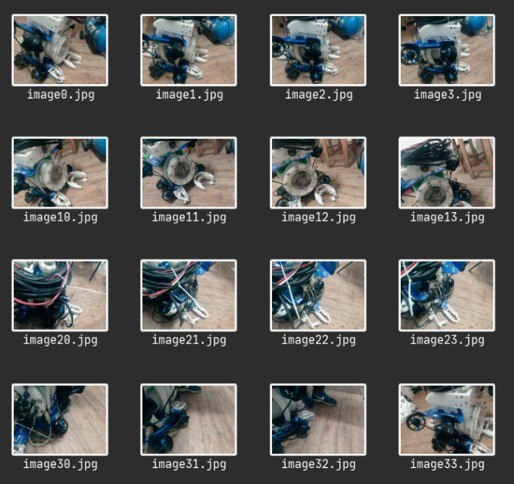
\includegraphics[width=0.3\textwidth]{"3d_task_figure2/input_images 2.jpg"}};
    \node[above=65pt, text width=100pt,align=center] at (figure1) {Samples from input images};
  
    % Second figure
    \node[draw, rectangle, blue, fill=blue!20] (figure2) at (4,2) {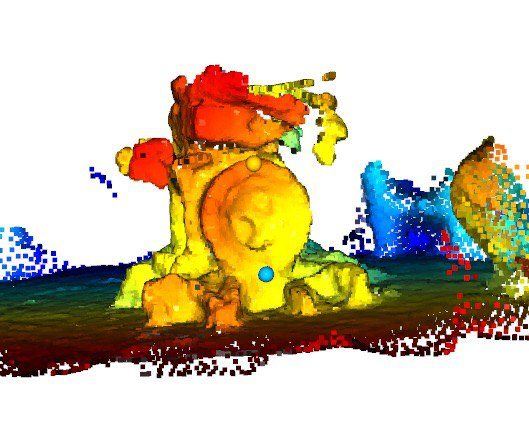
\includegraphics[width=0.25\textwidth]{3d_task_figure1/reference 2.jpg}};
    \node[above=50pt, text width=100pt,align=center] at (figure2) {Dense reconstruction Output};
  
    % Third figure
    \node[draw, rectangle, blue, fill=blue!20] (figure3) at (8,4) {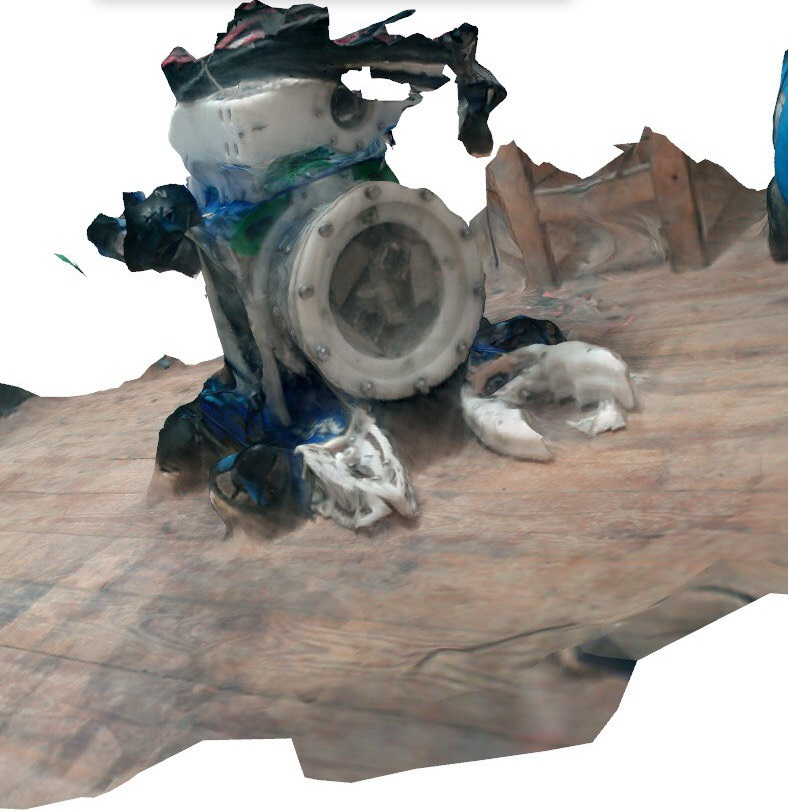
\includegraphics[width=0.27\textwidth]{3d_task_figure2/op1.jpg}};
    \node[above=50pt,text width=100pt,align=center] at (figure3) {Texture Output from different views};
  
    % third figure
    \node[draw, rectangle, blue, fill=blue!20] (figure4) at (8,0) {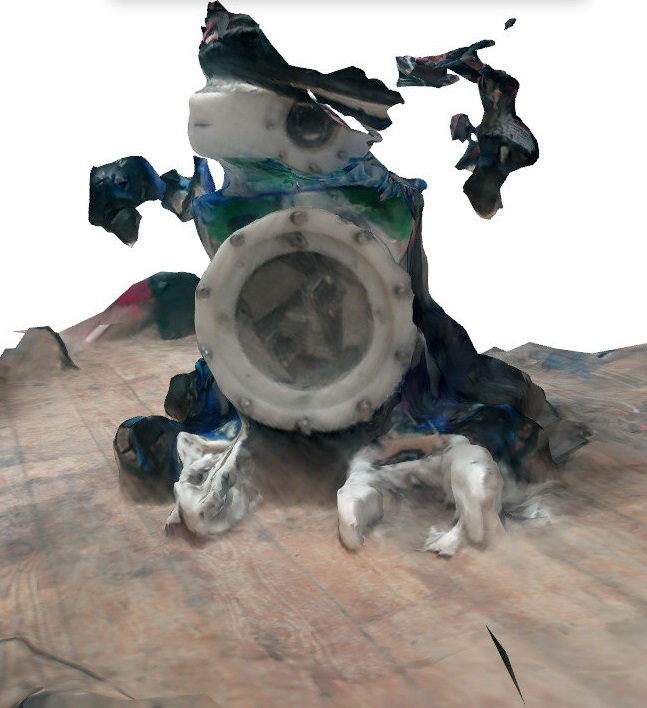
\includegraphics[width=0.27\textwidth]{3d_task_figure2/op2.jpg}};
    
    % Arrow between figures
    \draw[->, line width=1.3pt, blue] (figure1) -- (figure2);
    \draw[->, line width=1.3pt, blue] (figure2) -- (figure3);
    \draw[->, line width=1.3pt, blue] (figure2) -- (figure4);
  \end{tikzpicture}
  \caption{Reconstruction process}
  \label{fig:reconstruction}
  \end{figure}


\subsection*{Dimentions measurement procedures}
Draven measures specific dimensions in real time through a Graphical User Interface (GUI) using a Stereo Camera. These measurements can be saved as references on a 3D model for further dimension evaluations, as depicted in Figure \ref{fig:measurement}.

\begin{figure}[h]
  \centering
\begin{tikzpicture}
  % First figure
  \node[draw, rectangle, blue, fill=blue!20] (figure1) at (0,0) {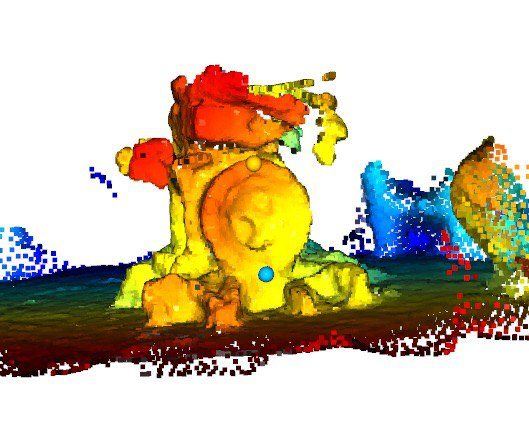
\includegraphics[width=0.25\textwidth]{3d_task_figure1/reference 2.jpg}};
  \node[above=40pt, text width=3cm,align=center] at (figure1) {Known size reference};

  % Second figure
  \node[draw, rectangle, blue, fill=blue!20] (figure2) at (4,0) {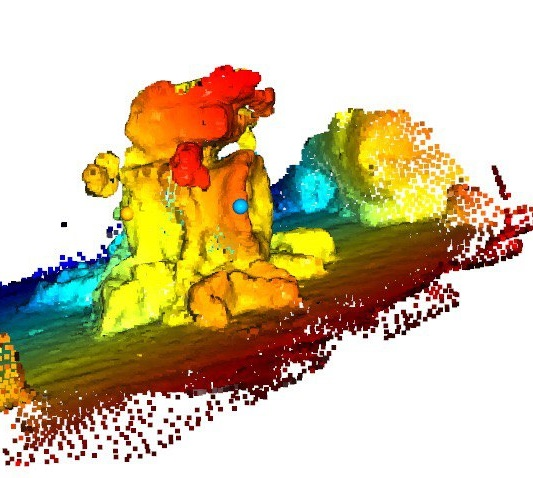
\includegraphics[width=0.25\textwidth]{3d_task_figure1/distance to be measured 2.jpg}};
  \node[above=40pt, text width=100pt,align=center] at (figure2) {Distance to be measured};

  % Third figure
  \node[draw, rectangle, blue, fill=blue!20] (figure3) at (8,0) {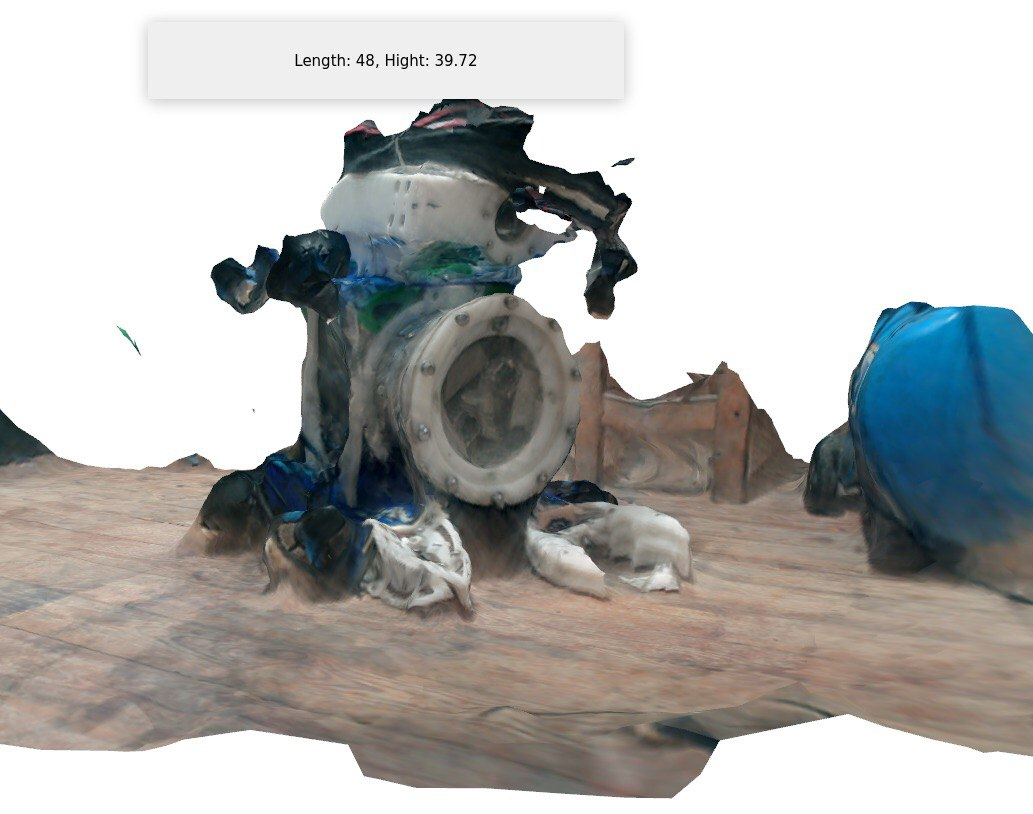
\includegraphics[width=0.32\textwidth]{3d_task_figure1/measurement_output 2.jpg}};
  \node[above=60pt,text width=100pt,align=center] at (figure3) {Measured distance labeled on the model};

  % Arrow between figures
  \draw[->, line width=1.3pt, blue] (figure1) -- (figure2);
  \draw[->, line width=1.3pt, blue] (figure2) -- (figure3);

\end{tikzpicture}
\caption{Measuring process}
\label{fig:measurement}
\end{figure}
\end{document}
